Radiative transfer theory describes how radiation that interacts with
hydrometeors produces an electromagnetic signal in satellite observations. Since
the purpose of the observations is to provide information on the physical
properties of hydrometeors, a way must be found to relate the observations to
those properties. This process is referred to as retrieval. This chapter
presents the mathematical formulation of the retrieval problem and provides a
brief introduction to the machine-learning-based methods to solve it.

\section{The retrieval problem}
\label{sec:machine_learning:retrieval_problem}

% So how can these observations be turned
%into estimates of physical properties? This is not a simple task because the
%observations are typically affected by non-negligible measurement noise and,
%more importantly, are generally ambiguous in the sense that physically different
%atmospheric states can produce nearly identical observations.

Mathematically, the problem of determining properties of hydrometeors from
satellite observations can be formulated as finding a state vector%
\footnote{ The notation for the state and observation vectors was deliberately
chosen to be the opposite of the conventions of inverse problem theory to make
it consistent with the conventions used in machine learning. }
$\vec{y} \in \mathrm{R}^{n}$ that describes the physical properties of the atmosphere from a
vector of observations $\vec{x} \in \mathrm{R}^{m}$. This so-called
\textit{retrieval problem} can be solved using the mathematical framework of
inverse problem theory. In inverse problem theory, the underlying assumption is
that the observations $\vec{x}$ are generated by a physical processes, which
can be described using a forward model function $f: \mathrm{R}^n \rightarrow
\mathrm{R}^m$, but may be affected by a random error $\vec{\epsilon} \in
\mathrm{R}^M$:
\begin{align}\label{eq:inverse_problem}
  \vec{x} &= f(\vec{y}) + \vec{\epsilon}
\end{align}

An exact solution to this problem does not exist. Because of the random noise
$\vec{\epsilon}$, the equation can never be strictly satisfied. Furthermore,
there usually exist many states $\vec{y}$ that produce similar measurements
$\vec{x}$, thus rendering the problem underconstrained. Since it does not
admit a unique solution, the retrieval problem is \textit{ill-posed}.

Although an exact solution to the retrieval problem is not possible, Bayesian
statistics provides a framework to extract the available information from the
observations. In the Bayesian approach, both the observations $\vec{x}$ and the
atmospheric state vector $\vec{y}$ are assumed to be random variables.
Furthermore,  it is assumed that $\vec{y}$ is distributed according to a known
\textit{a priori} distribution $p(\vec{y})$. Instead of a single, unique state
$\vec{y}$, the solution of the problem then becomes the \textit{a posteriori} (or
\textit{posterior}) distribution $p(\vec{y} | \vec{x})$ of the atmospheric
state. According to Bayes theorem, the a posteriori distribution for given
observations $\vec{x}$ is given by
\begin{align}\label{eq:bayes}
  p(\vec{y} | \vec{x}) &= \frac{p(\vec{x}|\vec{y})
  p(\vec{y})}{p(\vec{x})}.
\end{align}
Traditionally, Bayesian methods for solving the retrieval problem make use of
the right-hand side of Eq.~\ref{eq:bayes} to approximate the posterior
distribution. The approach pursued in this thesis is to learn the posterior
distributions $p(\vec{y}|\vec{x})$ directly from data. How this can be done is
the topic of the remainder of this chapter.

\section{Machine learning}


The field of machine learning is concerned with the development of algorithms
that can learn to solve computational tasks from data. More specifically, the
methods considered here solve the problem of \textit{supervised learning}. In
supervised learning, the task is to learn how to produce a certain output
$\vec{y}$ from inputs $\vec{x}$ given a set of pairs $\{(x_i, y_i)\}\text{ for
}i = 1, \ldots, N$ of specific input values $\vec{x}_i$ and corresponding output
values $\vec{y}_i$. In general, the inputs $\vec{x}$ and outputs $\vec{y}$ may
represent anything from simple numbers to images or texts. For the applications
considered here, the inputs are typically satellite images, and the outputs are
the corresponding physical quantities to be retrieved.

Machine learning has gone through a wave of immense popularity during the 2010s
triggered by the success of \textit{deep learning} methods in addressing a range
of computational problems in computer vision, natural language processing, and
artificial intelligence. The idea behind deep learning is to construct
increasingly powerful models from a hierarchy of simple models. Given sufficient
data, these models can learn highly complex relationships and require less
guidance from human experts to achieve good performance.

\subsection{Shallow machine learning}

Although the focus of this thesis is deep learning, this section will use a very
shallow model to illustrate the basic principles of machine-learning-based
remote sensing retrievals. The considered example tries to estimate rain at the
surface from infrared (IR) observations at a wavelength of $\lambda =
\SI{10.3}{\micro \meter}$. The training data, which contains of the in- and
outputs from which a solution to the retrieval problem should be learned, is
derived from co-locations of observations from the GOES 16 geostationary
satellite and the combined radar and passive microwave retrievals from the GPM
core observatory (see Sec. \ref{sec:radiative_transfer:synergies}).

The input $x$ for this particular example corresponds to the measured radiation
at a single pixel of the geostationary observations while the output $y$ is
given by the rain rate measured by the GPM core observatory. The retrieval
assumes a linear relationship between the observations $x$ and the rain rate $y$
in order to determine the precipitation corresponding to the geostationary
observations:
\begin{align}
  y &= a x + b
\end{align}
The two parameters of the linear regression model are the slope $a$ and 
the intercept $b$. They can be determined by finding the values that minimize the
squared error between the predictions and the true rain rates.

Panel (a) in Fig.~\ref{fig:machine_learning:linear_regression} shows the
distribution of the training data together with the learned relationship between
input and output data. This view reveals that the relationship is not very
robust, which becomes even clearer when the retrieval results (panel (b)) are
compared to the reference precipitation (panel (c)). The linear regression model
simply predicts rain almost everywhere where there is a cloud but completely
fails to reproduce the structure in the reference precipitation.

\begin{figure}
  \centering
  \includegraphics[width=\textwidth]{linear_regression.png}
  \caption{Example of a very simple precipitation retrieval. Panel (a) shows a
    density plot of the distribution of the input-output pairs, which consist of
    IR brightness temperatures and surface precipitation rates. The white line
    shows the linear relationship between observations and rain rate obtained by
    linear regression. Panel (b) shows retrieved precipitation rates when the
    learned relationship is applied to real observations. Panel (c) shows the
    true precipitation rates as present in the training data. Because of the
    narrow swath of the GPM precipitation radar the precipitation is not known
    across the full scene. }
  \label{fig:machine_learning:linear_regression}
\end{figure}

Given the bad performance of the simple linear regression model, it is natural
to ask how a better-performing model can be found. In general, there are three
dimensions along which a machine learning model can be improved:
\begin{description}
\item[Model expressivity:] The model used in this example can only learn
  linear relationships between input and output. The range of mathematical functions
  that a model can represent is referred to as its \textit{expressivity}. Increasing
  the model expressivity enables it to learn  more complex relationships between
  the input and output.
\item[Amount of input information:] The scatter plot in panel (a) of
  Fig.~\ref{fig:machine_learning:linear_regression} shows that the problem of
  retrieving precipitation from infrared (IR) observations is highly degenerate. For any
  value of the observations, the training data contains a wide range of different precipitation
  values. This makes it impossible to assign a unique `right' precipitation rate
  to an observed brightness temperature. The degeneracy can be decreased by
  adding more information to the input. One way to achieve this, for example, is
  to add observations from other channels or information from neighboring
  pixels. Depending on the problem, this may provide  more flexibility
  to distinguish different precipitation rates to the model.
\item[Amount of data:] A machine learning model can only learn relationships
  that are sufficiently well represented in the training data. For more complex
  retrievals than this one, larger amounts of training data are crucial for good
  retrieval performance.
\end{description}

Traditionally, the difficulty in improving a machine learning model was that it
is not sufficient to just increase the model expressivity or the amount of input
information. Both measures increase the flexibility of the model and may
thus cause it to \textit{overfit}. Overfitting occurs when the
model learns spurious relations from the training data, which are not actually
representative of the true relationship between input and output. This typically
causes predictions on unseen data to deteriorate drastically. Overfitting can be
counteracted by artificially reducing the expressivity of the model, a process
that is called \textit{regularization}, as well as by increasing the amount of data
that is used to train the model. However, the time and computational resources
that are required for training typically increase with the amount of data. If
the  increase is too rapid, the amount of data that a machine learning model
can be trained on may be limited.

Because of this, machine learning models traditionally depend on careful tuning
to the task at hand. Especially the trade-off between model expressivity and the
amount of data that can be used to train it required a multi-disciplinary
approach that combined domain-specific knowledge with machine-learning
experience to develop a good-performing model. A particular difficulty of
shallow models was their inability to handle large inputs with low information
density, such as the pixels from an image. Providing a shallow model with too
many inputs typically makes the models prone to overfitting and more difficult
to train. This gave rise to the practice of \textit{feature engineering}, which
consists of manually designing input variables that encode high-level
information in task-specific input features.

It should be noted that the linear regression model used here is extremely
simple and that there exist shallow machine learning methods that would likely
work much better for this example. Nonetheless, the application is not totally
unrealistic, given that it is similar to early precipitation retrievals from
geostationary observations \citep{vicente98}. To overcome the limitations of the
linear regression, the model from \citet{vicente98} predicts precipitation in
log-space and uses weather model data to post-process the retrieval results.
Modified versions of this retrieval are still in operational use today
\citep{siqueira19}.

\subsection{Deep learning}

The example discussed above illustrated the limitations of very shallow machine
learning methods that deep learning aims to overcome. The essential promise of
deep learning is that it decouples the dimensions along which a machine learning
model can be improved. Deep learning models achieve high expressivity by
stacking a large number of simple models and maximizing the amount of input
data. Since the training time of deep learning methods scales linearly with the
amount of available data while the required memory remains constant, the
increased model expressivity can be balanced with large amounts of training
data. This enables deep learning models to learn highly complex relationships
from data without the risk of overfitting.

  \subsection{Neural networks}

  Seen from a more general perspective, the linear regression model considered
  above is just a transformation from the input $x$ into the output $y$ with a
  set of learnable parameters, in this case, the slope and intercept of the
  regression. A neural network is just a sequence of such parametrized
  transformations, which are referred to as \textit{layers}. Each layer
  transforms an input vector into an output vector, which is passed on to the
  next layer. The exact form of each transformation can be adapted through its
  parameters, which is done by minimizing an error metric over the training
  data.

  Defined in this way, every neural network also satisfies the definition of a
  layer. This allows any neural network to be used as a component within a
  larger network.

  %sAn important characteristic of this definition of a neural network is its
  %recurrence: A neural network is itself a transformation of an input vector
  %into an output vector and may thus be used as a layer in a larger network. At
  %the same time, however, this makes the definition of what exactly constitutes a
  %layer in a network somewhat arbitrary.

  \subsubsection{The multi-layer perceptron}

  Extending the simple linear regression model to accommodate for multiple in-
  and outputs yields one of the most fundamental transformations used in neural
  networks. It is typically referred to as \textit{linear} or \textit{fully-} or
  \textit{densely-connected} layer. Mathematically, this layer implements an
  affine transformation of the input vector $\bm{x}$ of the form
  \begin{align}
    \bm{y} = \bm{W}x + \bm{b}
  \end{align}
  where $\bm{W} \in \mathrm{R}^{m \times n}$ is a matrix of weights $W_{i,j}$,
  and $\bm{b} \in \mathrm{R}^m$ a vector of  biases.

  Fully-connected layers are typically used in combination with a non-linear
  function that is applied element-wise to its inputs. These functions are
  called \textit{activation functions}. Without them, stacking fully-connected
  layers does not increase the expressivity of the neural network, which in this
  case depends only on the number of input and output variables.

  There exist a wide range of activation functions. One of the currently most
  commonly used activation functions in deep neural networks is the Rectified
  Linear Unit (ReLU).
  \begin{align}
    \text{ReLU(x)} = \begin{cases}
      x & x > 0 \\
      0 & x \leq 0
    \end{cases}
  \end{align}
  It should be noted, however, that neural network architectures are an area of
  active research and several alternatives and modifications of the ReLU
  activation have been proposed.

  A neural network consisting of one or several layers of fully-connected
  layers followed by activation functions is typically referred to as
  multi-layer perceptron (MLP). Since all numeric inputs can be brought into
  vector form and thus fed into an MLP, the MLP is one of the most fundamental
  forms of neural networks.

\subsubsection{Convolutional neural networks}

Although MLPs can be applied to image data directly by flattening the input into
a single vector, this approach was found to not work well in practice. The
principal reason for this is that the number of parameters in the model becomes
very large, making it prone to overfitting and the training more
difficult.

An important technique in the application of neural networks to image data was
the introduction of the convolutional layer, which replaces the
matrix multiplication of the fully-connected layer by a convolution with a
learnable filter kernel. Let $\bm{X} = [X_{i, j}]$ for $i = 1, \dots, M, j = 1,
\ldots, N$ be an input image of size $M \times N$ and $\bm{K} = [K_{i, j}]$ for
$i = - k \ldots k, j = -k, \ldots, k$ a given convolution kernel of 
size $(2k + 1) \tims (2k + 1)$. In two dimensions, the convolution
operation $\bm{Y} = \bm{X} * \bm{K}$ of
$\bm{X}$ and $K$ used in machine learning is defined as
\begin{align}\label{eq:machine_learning:convolution}
  Y_{i, j} &= \sum_{l=-k}^{k} \sum_{m=-k}^{k} X_{i + l, j + m} K_{i + l, j + m}
\end{align}
This operation corresponds to a filter mask whose response is calculated for all
possible locations in the input image by sliding the filter window across the
width and height of the image. Since digital images, as well as satellite
observations, contain information also along a spectral dimension, the images
actually correspond to three-dimensional tensors with an additional channel
dimension in addition to the two spatial dimensions. To account for this, the
kernel and sum in Eq.~\ref{eq:machine_learning:convolution} are extended across
all channels of the input image.

An illustration of the convolution operation for an input image with multiple
channels is shown Fig.~\ref{fig:machine_learning:convoluation}. The input
corresponds to a rank-three tensor with one channel and two spatial dimensions.
The kernel is limited in its extent in the spatial dimensions but extends over
all channels of the input. A two-dimensional output tensor is obtained by
calculating the kernel activation for all possible locations in the input
tensor. A convolutional layer consists of a set of convolution
kernels. The two-dimensional filter responses of each kernel are stacked along
the channel dimension to produce a rank-three tensor as output of the layer.

In a convolution layer, the convolution operation is typically combined with
the application of a bias term to each element in the output tensor. The learnable
parameters of a convolution layer thus correspond to the elements of each of its
kernels as well as the bias terms for each output.

\begin{figure}
  \centering
  \includegraphics[width=0.5\textwidth]{convolution}
  \caption{
    Illustration of the convolution operation. The output of the convolution
    operation is obtained by applying the filter kernel sequentially to every
    possible position in the input image.
  }
  \label{fig:machine_learning:convoluation}
\end{figure}

Since the convolution transformation is linear, it is a special case of the
fully-connected transformation of the corresponding flattened input image.
However, in the fully-connected case, each pixel in the output image would be
connected by independent parameters to all pixels in the input image, whereas
for the convolutional layers, the parameters are shared between all pixels in a
given channel of the output image. This greatly reduces the number of learnable
parameters of the convolutional layer compared to a fully-connected one.

The convolution encodes two important properties of images into the neural
network model, which are translation invariance and locality. Translation
invariance refers to the property of the convolution operation that its output
is independent of the relative location within the image. It is clear that this
is a suitable assumption for many image processing tasks since features that
identify an object should not be affected by their position in an image. The
property of locality refers to the fact that each output of a convolution layer
is determined only by a limited, connected subset of pixels of the input image,
the number of which depends on the kernel size $k$. This encodes the assumption
that for understanding the content of a given image region only neighboring
pixels should be relevant.

Convolutional neural networks are neural networks built-up of convolution
layers. These networks typically combine convolutional layers with downsampling
layers that successively decrease the size of the input image, which allows these
networks to combine information across the spatial dimensions of the image.

The motivation for this is to allow the model to learn a hierarchy of
transformations from low-level information on the pixel scale to a reduced
amount of high-level information that is relevant to the task that the
network is being trained to solve.

\subsubsection{Training}
%Now that the basic building blocks of modern neural networks have been
%introduced, the question remains how they can be trained to solve a given
%computational task. As mentioned above, we are considering the case of
%supervised learning in which training data in the form of samples from the joint
%distribution of input data $x$ and corresponding outputs $y$ are available.

The basic training approach for neural networks is similar to that of the
fitting of the parameters of a linear regression model, which are found by
minimizing a certain loss criterion over the training data. For linear
regression, this is typically the mean squared error, which can also be used to
train neural networks. In contrast to linear regression, however, the parameter
optimization for the neural network can not be solved explicitly. Instead,
neural networks rely on iterative minimization of the loss function using
gradient descent optimization.

While naive gradient descent would require traversing the whole training dataset
to compute the gradients required to perform a single descent step, it is in
practice sufficient and even beneficial to only use a small subset of samples
from the training data. This modification of traditional gradient descent, which
is known as \textit{stochastic (mini-batch) gradient descent}, allows neural
networks to scale  to very large datasets. In addition to that, the
stochasticity of the calculated gradients prevents the optimization process from
getting stuck in local minima of the cost function.

\subsubsection{Uncertainty in machine learning}

The ill-posed character of the retrieval problem discussed in
Sec. \ref{sec:machine_learning:retrieval_problem} leads to significant
uncertainties in most remote sensing retrievals. In addition to that,
the machine learning approach gives rise to two additional sources
of uncertainties in the retrieval.

%Machine learning techniques allow us to train a model that retrieved physical
%quantities from satellite observations. However, as discussed in
%Sec.~\ref{sec:remote_sensing:retrieval_probem}, there is no unique solution to
%the retrieval problem. Mathematically, this means that any prediction consisting
%of just a single value will always be wrong. Given the impossibility of solving
%the retrieval problem exactly and import questionj becomes whether the model
%learn how wrong it is?

The total error that a machine learning model makes in its prediction is its
\textit{predictive uncertainty}. The predictive uncertainty can be decomposed
into three independent sources. The first one, referred to as \textit{epistemic
  uncertainty}, is the uncertainty caused by a lack of training data. Its
defining property is that it can be reduced by collecting more data to train the
model on. The second type is called \textit{aleatoric uncertainty}. This
uncertainty refers to the uncertainty that cannot be reduced by increasing the
amount of data that the model is trained on. In the context of satellite
observations, this uncertainty is caused by the inability of the observations to
fully determine the observed atmospheric state. It is thus a consequence of the
ill-posed nature of the retrieval problem  discussed in
Sec.~\ref{sec:machine_learning:retrieval_problem}.

An illustration of the concepts of aleatoric and epistemic uncertainty is provided
in Fig.~\ref{fig:machine_learning:uncertainties}. The plot shows the joint
distribution of observations and the retrieval target for a hypothetical retrieval
scenario. The filled contours in the background show the actual joint distribution
that relates the observations to the targets. The grey markers show the
available training samples. If these samples were to be used to train a neural
network model, the uncertainty in the left part of the graph would be dominated
by the aleatoric uncertainty, because the spread of the underlying, true relationship
is well represented in the training data. In the right part of the graph,
however, the training samples are too few to capture the relevant features of
the relationship and uncertainties would be dominated by epistemic uncertainty.

\begin{figure}
  \centering
  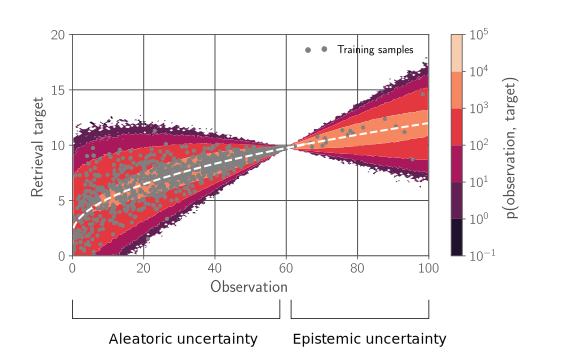
\includegraphics[width=\textwidth]{uncertainties}
  \caption{
    Illustration of aleatoric and epistemic uncertainty. The graph
    displays the relationship between observations and retrieval target
    for a hypothetical retrieval scenario. In the left part of graph the
    uncertainties are dominated by aleatoric uncertainty, whereas in
    the right part they are dominated by epistemic uncertainty.
  }
  \label{fig:machine_learning:uncertainties}
\end{figure}

The final source of uncertainty is caused by differences between the training
data and the data that the model is actually applied on. It is typically
referred to as \textit{covariate shift}. It is obvious that when the wrong data
is used to train the model, it is likely to produce wrong results. However,
subtle changes between training data and the actual data that the model is
applied on are not uncommon and can  increase the predictive uncertainty of
the model.

\subsection{Revisiting the precipitation retrieval}

To provide a demonstration of the capabilities of the deep learning methods,
Fig.~\ref{fig:machine_learning:retrieval_comparison} revisits
the retrieval example introduced above and displays the results from two additional
retrievals, which have been trained using the same data.

The first one is based on an MLP, which uses the same single-pixel input as the
linear regression model. The results from this retrieval are shown in panel (b).
Compared to the reference precipitation shown in panel (d), the results show
modest improvements in the structure of the precipitation, but its spatial
extent is still strongly overestimated. Since the MLP uses only information from
a single input channel, it is severely limited in the relations that it can
learn. It is therefore not surprising that it does not work much better than the
linear regression model.

To explore the full potential of deep learning methods, the second model uses a
CNN to retrieve precipitation using the full input image and all 16 channels of
the geostationary observations simultaneously. These results show clear
improvements both in the structure of the retrieved precipitation as well as its
spatial extent.

\begin{figure}
  \centering
\includegraphics[width=\textwidth]{retrieval_comparison}
\caption{Retrieved precipitation from a linear regression model
  (panel (a)), an MLP applied separately to each input pixel
  (panel (b)) and a CNN that predicts precipitation for the
  full input image using all available channels (panel (c)).
  The reference precipitation measured by the combined radar
  and passive microwave retrievals of the GPM core observatory
  are shown in panel (d).}
\label{fig:machine_learning:retrieval_comparison}
\end{figure}

This example clearly demonstrates the ability of deep learning techniques to
improve remote sensing retrievals. However, it should also be noted that the
computational effort required to train these models increases by orders of
magnitude. The simple linear regression model used here takes at most a few
seconds to train. The training of the MLP and CNN models, on the other hand,
takes hours respectively days and uses dedicated computing hardware. This is in
general not an issue because the training is a one-time effort and the
evaluation of the model is much faster, but nonetheless a fact that deserves
consideration.

The results in Fig.~\ref{fig:machine_learning:retrieval_comparison} show that
even the more advanced retrieval model fails to truthfully reproduce the
precipitation in the reference data. Since VIS and IR observations from
geostationary satellites are only sensitive to the upper parts of the clouds,
the inputs provided to the retrieval are only indirectly related to
precipitation at the surface. The ill-posed character of the retrieval problem
dictates that any specific prediction from a neural network will be wrong. Given
this fundamental nature of remote sensing retrievals, the next section explores
how neural networks can learn how wrong they expect to be.


\section{Handling uncertainty in remote sensing retrievals}

One of the issues that this thesis aims to address is the quantification of
retrieval uncertainties in machine-learning-based remote sensing retrievals. The
two methods that were explored in the appended studies fall into the category of
probabilistic regression methods. This means that they account for the aleatoric
uncertainty in the prediction but neglect epistemic uncertainty and covariate
shift. Below, these two approaches are presented followed by a discussion of
other approaches for quantifying uncertainties in neural network predictions.

\subsection{Probabilistic regression}

Aleatoric uncertainty arises due to ambiguous samples in the training data. The
fact that these ambiguities are represented in the training data means that they
can be predicted by a suitably trained neural network model. To allow for this,
the deterministic formulation of regression, i.e. to predict a single value $y =
f(\vec{x})$, is replaced by a probabilistic formulation, which aims predict the
probability distribution $p(y|\vec{x})$ of $y$ given the input vector $\vec{x}$.

\subsubsection{Quantile regression neural networks}

%To predict a distribution $p(y|x)$ the neural network model can trained
%to predict parameters of a parametrized probability distribution and
%an optimization criterion for the training can be obtained by maximizing the
%likelihood of the training samples under the predicted distribution. Assuming
%$p(y|x)$ to be Gaussian distributed with mean $\mu = f(x)$ and constant standard
%deviation yields a training criterion equivalent to the MSE loss.

Quantile regression neural networks (QRNNs) predict the distribution
$p(y|\vec{x})$ for a scalar output $y$ using a sequence of its quantiles. Given
a fraction $\tau \in [0, 1]$, the corresponding quantile $y_\tau$ is defined as
\begin{align}
  y_\tau &= F^{-1}(\tau)
\end{align}
with $F(y) = \int_{-\infty}^y p(y|\vec{x})\ dy$ the cumulative distribution
function (CDF) of the distribution $p(y|\vec{x})$. A neural network can learn to predict a quantile
$y_\tau$ by training it to minimize the quantile loss
\begin{align}
  \mathcal{L}(y_\tau, y) &=
  \begin{cases}
    \tau  |y_\tau - y| & \text{if } y > y_\tau \\
    (1 - \tau)  |y_\tau - y| & \text{otherwise} \\
    \end{cases}
\end{align}
where $y_\tau$ is the predicted quantile and $y$ is the reference output value
from the training data. It is important to realize here  that $y$ is only
required to be an ordinary sample of the distribution $p(y|\vec{x})$ and does not
require the distribution $p(y|\vec{x})$ to be explicitly represented in the
training data.

The approach can be extended to the prediction of multiple quantiles
corresponding to a sequence of quantile fractions $\mathrm{T} = \{\tau_1,
\ldots, \tau_N\}$ by training the network to minimize the sum of the quantile
losses
\begin{align}
  \mathcal{L}_\mathrm{T}(\vec{y}_T, y) &= 
  \sum_{\tau \in \mathrm{T}} \mathcal{L}_\tau(y_\tau, y)
\end{align}
where now $\vec{y}_T = [y_{\tau_1}, \ldots, y_{\tau_N}]$ is a vector of predicted quantiles.

The basic principle of QRNNs is illustrated
Fig.~\ref{fig:machine_learning:qrnn}. To predict the distribution of a scalar
variable $y$ conditioned on a vector of inputs $\vec{x}$, QRNNs use a neural
network to transform the vector of inputs into a vector of outputs. The outputs
correspond to a sequence of quantiles, which can be used to derive a piece-wise
linear approximation of the CDF of $p(y|\vec{x})$.

\begin{figure}[btp]
  \centering
  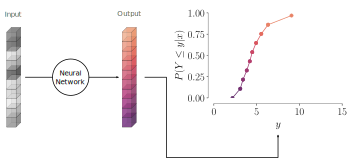
\includegraphics[width=.75\textwidth]{qrnn.pdf}
  \caption{Basic principle of QRNNS. QRNNs predict the distribution of
    a scalar output variable $y$ using a vector of quantiles from which the
    an approximation of the CDF of the distribution can be constructed.}
  \label{fig:machine_learning:qrnn}
\end{figure}

Using quantiles to represent the distribution $p(y|\vec{x})$ has the advantage
that the neural network can learn the shape of the posterior distribution of the
retrieval. This is in contrast to other probabilistic regression methods, which
often impose a more constrained parametrized form of $p(y|x)$, such as a Gaussian
whose mean and standard deviation are predicted.

An unresolved issue with QRNNs is quantile crossing. There is nothing that
ensures that the quantiles predicted by a QRNN as they are employed here are in
increasing order. QRNNs can thus produce mathematically inconsistent
predictions, where quantiles of lower fractions exceed those of higher
fractions. However, at least for the applications considered in this thesis,
this was not found to be a critical issue.

\subsubsection{Density regression neural networks}

The second approach for predicting the distribution $p(y|\vec{x})$ is based on
the work by \citet{oord16} and \citet{sonderby20}. Since it has not been given
an explicit name by the authors, it is referred to here as density regression
neural networks (DRNNs). In this approach, the regression problem is cast as a
classification problem by discretizing the domain of output values $y$ into bins
$y_0, \ldots, y_n$ and then predicting for each bin the probability $p_i(y >=
y_{i - 1}, y < y_i)$ of the observed $y$ falling into the $i$th bin.

Mathematically this is implemented by minimizing the
categorical cross-entropy loss
\begin{align}
  \mathcal{L}(\hat{\vec{p}}, y) &=  -\log(\hat{p}_i) \text { with i such that } y_{i - 1} \leq y < y_i.
\end{align}
where $\hat{\vec{p}} = [\hat{p}_1, \ldots, \hat{p}_n]$ is a vector of predicted probabilities.

The predicted vector of bin probabilities can then be used as a piece-wise
constant approximation of the PDF of $p(y | \vec{x})$, as illustrated in
Fig.~\ref{fig:machine_learning:drnn}. Since the CDF of $p(y | \vec{x})$ can be
calculated from the PDF and vise versa, QRNNs and DRNNs are functionally very
similar. Compared to QRNNs, DRNNs have the advantage of avoiding quantile
crossing by construction. What may be a disadvantage of DRNNs is that they require
a relatively high number of outputs  when the values of $y$ vary across a wide
range.
\begin{figure}[btp]
  \centering
  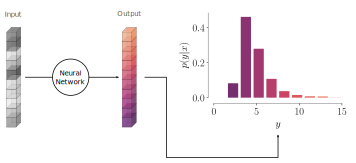
\includegraphics[width=.75\textwidth]{drnn.pdf}
  \caption{The basic functioning of QRNNS. QRNNs predict the distribution of
    a scalar output variable $y$ using a vector of quantiles from which the
    an approximation of the CDF of the distribution can be constructed.}
  \label{fig:machine_learning:drnn}
\end{figure}

\subsubsection{The aleatoric approximation}

Both QRNNs and DRNNs only learn to quantify the aleatoric uncertainty and
neglect epistemic uncertainty and covariate shift. It is thus necessary that the
aleatoric component of the predictive uncertainty dominates the two other types
of uncertainties for these models to produce reliable uncertainty estimates.
Given that remote sensing observations are produced in a controlled environment
and the range of possible observations is generally well understood, it is
usually possible to obtain large amounts of reliable training data, which
minimizes epistemic uncertainty and the effects of covariate shift. Given the
cost of designing and operating these observation systems, one should expect
that an effort is made to minimize both epistemic uncertainty and covariate
shift, thus leaving the aleatoric uncertainty as the only irreducible source of
uncertainty in the measurements. Additional, empirical evidence for the
usefulness of the aleatoric approximation comes from the results presented in
this thesis, where the probabilistic predictions from QRNNs and DRNNs were found
to provide reliable estimates of the retrieval uncertainty.

\subsubsection{Further limitations}

A further limitation of QRNNs and DRNNs is their handling of multiple retrieval
outputs. The formulations presented above were based on the assumption of a
scalar retrieval output $y$. These approaches can easily be extended to multiple
output variables by simply minimizing the mean of their individual losses. This
was found to work well in practice but provides no way of representing the
correlations between the multiple outputs in the results. QRNNs and DRNNs are
therefore not able to produce random samples  that accurately the correlations
between the output variables.

\subsection{Other approaches for quantifying uncertainties}

Because of their limitations, QRNNs and DRNNs may not be the best choice for all
applications. Therefore, the following section briefly reviews other approaches
for quantifying retrieval uncertainty and compares them to the probabilistic
regression approach.

\subsubsection{Bayesian neural networks}

Bayesian neural networks (BNNs) can handle both epistemic and aleatoric
uncertainty. For BNNs, not only the target $y$ is assumed to be a random
variable, but also the parameters $\vec{\theta}$ of the neural network model. The
random distribution of these parameters represents the uncertainty caused by the
limited amount of training data that the model is trained on. Instead of
learning specific parameters, a BNN learns a distribution of each of its
parameters.

A single prediction from a BNN $p(y|\vec{x}, \vec{\theta})$ for a specific input
$\vec{x}$ is obtained by sampling values of the model parameters from the learned
distributions and using them to evaluate the model. The epistemic uncertainty in
the model predictions is typically quantified by sampling multiple instances of
the model parameters $\vec{\theta}$ and evaluating the model for each of them. For
inputs $\vec{x}$ that the model has encountered often during training, the
distribution of $\vec{\theta}$ values will be sharp so that the distribution
$p(y|\vec{x}, \vec{\theta})$ does not change much for different realizations
of the model parameters $\vec{\theta}$. For
samples where this is not the case, there will be a larger spread and thus
higher epistemic uncertainty in the predictions.

Despite their ability to quantify both aleatoric and epistemic uncertainty, BNNs
have not yet found widespread adoption in practical applications. One reason for
this is likely that their training takes significantly more time. Another
disadvantage is that the quantification of epistemic uncertainty requires
evaluating the network multiple times. This typically increases the time
required to evaluate the model by an order of magnitude, which is a
disadvantage for applications that require high throughput.

Despite these potential disadvantages, \citet{orescanin22} have recently
demonstrated the application of Bayesian neural networks to the classification
of precipitation types and shown that the predicted uncertainties are
well-calibrated. They also found that the predictive uncertainty is dominated by
aleatoric uncertainty, which provides further evidence for the validity of
the aleatoric approximation.

\subsubsection{Generative models}

Generative models are another approach for quantifying uncertainties in neural
network predictions. Instead of predicting the conditional probability
distribution $p(\vec{y}|\vec{x})$ explicitly, these methods are trained to generate
samples from the distribution directly. These methods have gained popularity in
computer vision tasks due to their ability to generate samples from highly
complex probability distributions such as images of faces or generic objects.

The advantage of this approach is that it can handle spatial correlations in the
uncertainties, which is not the case for the other methods discussed so far.
This means that they can produce spatially coherent samples of the retrieved
variables that look very realistic. Recent work has explored the application of
generative models for short-term weather forecasting \citep{ravuri21} and
probabilistic downscaling of precipitation \citep{harris22, leinonen20}.
However, these models are also known to be more difficult and take longer to
train. In addition to that, they also need to be evaluated multiple times to
calculate statistics of the posterior distribution, which increases the
computational requirements of the retrieval.
